\documentclass[11pt,a4paper]{article}
\usepackage[T1]{fontenc}
\usepackage[utf8]{inputenc}
\usepackage{lmodern}
\usepackage[margin=2.4cm]{geometry}
\usepackage{xcolor,tikz,booktabs,graphicx,amsmath,caption,array,enumitem,microtype}
\usepackage[colorlinks=true,linkcolor=accent,urlcolor=accent,citecolor=accent]{hyperref}
\usetikzlibrary{arrows.meta,positioning}
\definecolor{ink}{HTML}{0B0B0B}
\definecolor{panel}{HTML}{F1F0EC}
\definecolor{accent}{HTML}{2A78D6}
\definecolor{second}{HTML}{EB6834}
\captionsetup{font=small,labelfont=bf}
\setlist{itemsep=2pt,topsep=4pt}
\setlength{\parskip}{5pt}
\setlength{\parindent}{0pt}
% Generated by `newsvar vol report`; do not edit.
\newcommand{\EarlierOpenCountGain}{+2.2\%}
\newcommand{\EarlierOpenCountPin}{+0.3\%}
\newcommand{\EarlierOpenCountT}{2.58}
\newcommand{\EarlierOpenExpected}{25.0}
\newcommand{\EarlierOpenExpectedOne}{5.0}
\newcommand{\EarlierOpenFzGain}{+0.0129}
\newcommand{\EarlierOpenGwP}{0.038}
\newcommand{\EarlierOpenHarBreaches}{26}
\newcommand{\EarlierOpenHarBreachesOne}{5}
\newcommand{\EarlierOpenHarFz}{-4.067}
\newcommand{\EarlierOpenHarKupiec}{0.84}
\newcommand{\EarlierOpenHarPin}{8.79}
\newcommand{\EarlierOpenHarQlike}{0.3222}
\newcommand{\EarlierOpenHarVsHsPin}{+12.1\%}
\newcommand{\EarlierOpenHsBreaches}{25}
\newcommand{\EarlierOpenHsBreachesOne}{11}
\newcommand{\EarlierOpenHsFz}{-3.901}
\newcommand{\EarlierOpenHsKupiec}{1.00}
\newcommand{\EarlierOpenHsPin}{10.00}
\newcommand{\EarlierOpenMeanSurpriseGain}{+0.2\%}
\newcommand{\EarlierOpenMeanSurprisePin}{+0.3\%}
\newcommand{\EarlierOpenMeanSurpriseT}{0.37}
\newcommand{\EarlierOpenN}{500}
\newcommand{\EarlierOpenPinGain}{+1.2\%}
\newcommand{\EarlierOpenPinT}{1.72}
\newcommand{\EarlierOpenQlikeGain}{+4.2\%}
\newcommand{\EarlierOpenQlikeP}{0.003}
\newcommand{\EarlierOpenQlikeT}{2.78}
\newcommand{\EarlierOpenShareLevelGain}{+1.3\%}
\newcommand{\EarlierOpenShareLevelPin}{+0.3\%}
\newcommand{\EarlierOpenShareLevelT}{1.58}
\newcommand{\EarlierOpenShareSurpriseGain}{+0.3\%}
\newcommand{\EarlierOpenShareSurprisePin}{+0.4\%}
\newcommand{\EarlierOpenShareSurpriseT}{0.46}
\newcommand{\EarlierOpenTextBreaches}{25}
\newcommand{\EarlierOpenTextBreachesOne}{5}
\newcommand{\EarlierOpenTextFz}{-4.079}
\newcommand{\EarlierOpenTextKupiec}{1.00}
\newcommand{\EarlierOpenTextPin}{8.69}
\newcommand{\EarlierOpenTextQlike}{0.3086}
\newcommand{\EarlierPreCountGain}{+2.8\%}
\newcommand{\EarlierPreCountPin}{+0.3\%}
\newcommand{\EarlierPreCountT}{2.69}
\newcommand{\EarlierPreExpected}{24.9}
\newcommand{\EarlierPreExpectedOne}{5.0}
\newcommand{\EarlierPreFzGain}{+0.0164}
\newcommand{\EarlierPreGwP}{0.027}
\newcommand{\EarlierPreHarBreaches}{20}
\newcommand{\EarlierPreHarBreachesOne}{5}
\newcommand{\EarlierPreHarFz}{-3.859}
\newcommand{\EarlierPreHarKupiec}{0.30}
\newcommand{\EarlierPreHarPin}{11.44}
\newcommand{\EarlierPreHarQlike}{0.4547}
\newcommand{\EarlierPreHarVsHsPin}{+6.2\%}
\newcommand{\EarlierPreHsBreaches}{30}
\newcommand{\EarlierPreHsBreachesOne}{10}
\newcommand{\EarlierPreHsFz}{-3.720}
\newcommand{\EarlierPreHsKupiec}{0.31}
\newcommand{\EarlierPreHsPin}{12.19}
\newcommand{\EarlierPreMeanSurpriseGain}{+2.6\%}
\newcommand{\EarlierPreMeanSurprisePin}{+1.2\%}
\newcommand{\EarlierPreMeanSurpriseT}{1.01}
\newcommand{\EarlierPreN}{498}
\newcommand{\EarlierPrePinGain}{+1.4\%}
\newcommand{\EarlierPrePinT}{1.59}
\newcommand{\EarlierPreQlikeGain}{+5.0\%}
\newcommand{\EarlierPreQlikeP}{0.015}
\newcommand{\EarlierPreQlikeT}{2.16}
\newcommand{\EarlierPreShareLevelGain}{+3.1\%}
\newcommand{\EarlierPreShareLevelPin}{+0.9\%}
\newcommand{\EarlierPreShareLevelT}{0.99}
\newcommand{\EarlierPreShareSurpriseGain}{+2.4\%}
\newcommand{\EarlierPreShareSurprisePin}{+1.3\%}
\newcommand{\EarlierPreShareSurpriseT}{0.89}
\newcommand{\EarlierPreTextBreaches}{20}
\newcommand{\EarlierPreTextBreachesOne}{5}
\newcommand{\EarlierPreTextFz}{-3.876}
\newcommand{\EarlierPreTextKupiec}{0.30}
\newcommand{\EarlierPreTextPin}{11.28}
\newcommand{\EarlierPreTextQlike}{0.4318}
\newcommand{\FreshOpenCountGain}{+1.3\%}
\newcommand{\FreshOpenCountPin}{-0.3\%}
\newcommand{\FreshOpenCountT}{0.93}
\newcommand{\FreshOpenExpected}{11.2}
\newcommand{\FreshOpenExpectedOne}{2.2}
\newcommand{\FreshOpenFzGain}{+0.0168}
\newcommand{\FreshOpenGwP}{0.607}
\newcommand{\FreshOpenHarBreaches}{8}
\newcommand{\FreshOpenHarBreachesOne}{2}
\newcommand{\FreshOpenHarFz}{-4.017}
\newcommand{\FreshOpenHarKupiec}{0.30}
\newcommand{\FreshOpenHarPin}{9.47}
\newcommand{\FreshOpenHarQlike}{0.3391}
\newcommand{\FreshOpenHarVsHsPin}{+4.9\%}
\newcommand{\FreshOpenHsBreaches}{13}
\newcommand{\FreshOpenHsBreachesOne}{4}
\newcommand{\FreshOpenHsFz}{-3.859}
\newcommand{\FreshOpenHsKupiec}{0.59}
\newcommand{\FreshOpenHsPin}{9.96}
\newcommand{\FreshOpenMeanSurpriseGain}{-1.2\%}
\newcommand{\FreshOpenMeanSurprisePin}{-0.5\%}
\newcommand{\FreshOpenMeanSurpriseT}{-1.05}
\newcommand{\FreshOpenN}{224}
\newcommand{\FreshOpenPinGain}{+1.6\%}
\newcommand{\FreshOpenPinT}{2.01}
\newcommand{\FreshOpenQlikeGain}{-1.7\%}
\newcommand{\FreshOpenQlikeP}{0.718}
\newcommand{\FreshOpenQlikeT}{-0.58}
\newcommand{\FreshOpenShareLevelGain}{-1.3\%}
\newcommand{\FreshOpenShareLevelPin}{-0.4\%}
\newcommand{\FreshOpenShareLevelT}{-0.95}
\newcommand{\FreshOpenShareSurpriseGain}{-1.3\%}
\newcommand{\FreshOpenShareSurprisePin}{-0.9\%}
\newcommand{\FreshOpenShareSurpriseT}{-1.16}
\newcommand{\FreshOpenTextBreaches}{8}
\newcommand{\FreshOpenTextBreachesOne}{3}
\newcommand{\FreshOpenTextFz}{-4.034}
\newcommand{\FreshOpenTextKupiec}{0.30}
\newcommand{\FreshOpenTextPin}{9.32}
\newcommand{\FreshOpenTextQlike}{0.3447}
\newcommand{\FreshPreCountGain}{-1.0\%}
\newcommand{\FreshPreCountPin}{+0.3\%}
\newcommand{\FreshPreCountT}{-0.59}
\newcommand{\FreshPreExpected}{11.2}
\newcommand{\FreshPreExpectedOne}{2.2}
\newcommand{\FreshPreFzGain}{+0.0152}
\newcommand{\FreshPreGwP}{0.106}
\newcommand{\FreshPreHarBreaches}{7}
\newcommand{\FreshPreHarBreachesOne}{3}
\newcommand{\FreshPreHarFz}{-3.803}
\newcommand{\FreshPreHarKupiec}{0.17}
\newcommand{\FreshPreHarPin}{11.28}
\newcommand{\FreshPreHarQlike}{0.3364}
\newcommand{\FreshPreHarVsHsPin}{+1.3\%}
\newcommand{\FreshPreHsBreaches}{12}
\newcommand{\FreshPreHsBreachesOne}{5}
\newcommand{\FreshPreHsFz}{-3.736}
\newcommand{\FreshPreHsKupiec}{0.81}
\newcommand{\FreshPreHsPin}{11.43}
\newcommand{\FreshPreMeanSurpriseGain}{+0.1\%}
\newcommand{\FreshPreMeanSurprisePin}{-0.5\%}
\newcommand{\FreshPreMeanSurpriseT}{0.05}
\newcommand{\FreshPreN}{224}
\newcommand{\FreshPrePinGain}{+1.8\%}
\newcommand{\FreshPrePinT}{1.15}
\newcommand{\FreshPreQlikeGain}{+4.3\%}
\newcommand{\FreshPreQlikeP}{0.042}
\newcommand{\FreshPreQlikeT}{1.72}
\newcommand{\FreshPreShareLevelGain}{+1.1\%}
\newcommand{\FreshPreShareLevelPin}{-0.5\%}
\newcommand{\FreshPreShareLevelT}{0.47}
\newcommand{\FreshPreShareSurpriseGain}{+0.6\%}
\newcommand{\FreshPreShareSurprisePin}{-0.5\%}
\newcommand{\FreshPreShareSurpriseT}{0.29}
\newcommand{\FreshPreTextBreaches}{10}
\newcommand{\FreshPreTextBreachesOne}{3}
\newcommand{\FreshPreTextFz}{-3.818}
\newcommand{\FreshPreTextKupiec}{0.71}
\newcommand{\FreshPreTextPin}{11.09}
\newcommand{\FreshPreTextQlike}{0.3221}
\newcommand{\FreshStart}{2026-01-02}
\newcommand{\HOneP}{0.003}
\newcommand{\HTwoP}{0.043}
\newcommand{\HoldOpenCountGain}{+1.9\%}
\newcommand{\HoldOpenCountPin}{+0.1\%}
\newcommand{\HoldOpenCountT}{2.62}
\newcommand{\HoldOpenExpected}{36.2}
\newcommand{\HoldOpenExpectedOne}{7.2}
\newcommand{\HoldOpenFzGain}{+0.0141}
\newcommand{\HoldOpenGwP}{0.028}
\newcommand{\HoldOpenHarBreaches}{34}
\newcommand{\HoldOpenHarBreachesOne}{7}
\newcommand{\HoldOpenHarFz}{-4.051}
\newcommand{\HoldOpenHarKupiec}{0.70}
\newcommand{\HoldOpenHarPin}{9.00}
\newcommand{\HoldOpenHarQlike}{0.3274}
\newcommand{\HoldOpenHarVsHsPin}{+9.9\%}
\newcommand{\HoldOpenHsBreaches}{38}
\newcommand{\HoldOpenHsBreachesOne}{15}
\newcommand{\HoldOpenHsFz}{-3.888}
\newcommand{\HoldOpenHsKupiec}{0.76}
\newcommand{\HoldOpenHsPin}{9.99}
\newcommand{\HoldOpenMeanSurpriseGain}{-0.2\%}
\newcommand{\HoldOpenMeanSurprisePin}{+0.1\%}
\newcommand{\HoldOpenMeanSurpriseT}{-0.41}
\newcommand{\HoldOpenN}{724}
\newcommand{\HoldOpenPinGain}{+1.3\%}
\newcommand{\HoldOpenPinT}{2.46}
\newcommand{\HoldOpenQlikeGain}{+2.3\%}
\newcommand{\HoldOpenQlikeP}{0.045}
\newcommand{\HoldOpenQlikeT}{1.69}
\newcommand{\HoldOpenShareLevelGain}{+0.4\%}
\newcommand{\HoldOpenShareLevelPin}{+0.0\%}
\newcommand{\HoldOpenShareLevelT}{0.64}
\newcommand{\HoldOpenShareSurpriseGain}{-0.2\%}
\newcommand{\HoldOpenShareSurprisePin}{-0.0\%}
\newcommand{\HoldOpenShareSurpriseT}{-0.35}
\newcommand{\HoldOpenTextBreaches}{33}
\newcommand{\HoldOpenTextBreachesOne}{8}
\newcommand{\HoldOpenTextFz}{-4.065}
\newcommand{\HoldOpenTextKupiec}{0.58}
\newcommand{\HoldOpenTextPin}{8.89}
\newcommand{\HoldOpenTextQlike}{0.3198}
\newcommand{\HoldPreCountGain}{+1.9\%}
\newcommand{\HoldPreCountPin}{+0.3\%}
\newcommand{\HoldPreCountT}{2.08}
\newcommand{\HoldPreExpected}{36.1}
\newcommand{\HoldPreExpectedOne}{7.2}
\newcommand{\HoldPreFzGain}{+0.0160}
\newcommand{\HoldPreGwP}{0.004}
\newcommand{\HoldPreHarBreaches}{27}
\newcommand{\HoldPreHarBreachesOne}{8}
\newcommand{\HoldPreHarFz}{-3.842}
\newcommand{\HoldPreHarKupiec}{0.10}
\newcommand{\HoldPreHarPin}{11.39}
\newcommand{\HoldPreHarQlike}{0.4180}
\newcommand{\HoldPreHarVsHsPin}{+4.7\%}
\newcommand{\HoldPreHsBreaches}{42}
\newcommand{\HoldPreHsBreachesOne}{15}
\newcommand{\HoldPreHsFz}{-3.725}
\newcommand{\HoldPreHsKupiec}{0.33}
\newcommand{\HoldPreHsPin}{11.95}
\newcommand{\HoldPreMeanSurpriseGain}{+2.0\%}
\newcommand{\HoldPreMeanSurprisePin}{+0.7\%}
\newcommand{\HoldPreMeanSurpriseT}{0.98}
\newcommand{\HoldPreN}{722}
\newcommand{\HoldPrePinGain}{+1.5\%}
\newcommand{\HoldPrePinT}{1.98}
\newcommand{\HoldPreQlikeGain}{+4.8\%}
\newcommand{\HoldPreQlikeP}{0.005}
\newcommand{\HoldPreQlikeT}{2.58}
\newcommand{\HoldPreShareLevelGain}{+2.6\%}
\newcommand{\HoldPreShareLevelPin}{+0.5\%}
\newcommand{\HoldPreShareLevelT}{1.06}
\newcommand{\HoldPreShareSurpriseGain}{+1.9\%}
\newcommand{\HoldPreShareSurprisePin}{+0.7\%}
\newcommand{\HoldPreShareSurpriseT}{0.92}
\newcommand{\HoldPreTextBreaches}{30}
\newcommand{\HoldPreTextBreachesOne}{8}
\newcommand{\HoldPreTextFz}{-3.858}
\newcommand{\HoldPreTextKupiec}{0.28}
\newcommand{\HoldPreTextPin}{11.22}
\newcommand{\HoldPreTextQlike}{0.3978}
\newcommand{\HoldoutEnd}{2026-11-20}
\newcommand{\HoldoutStart}{2023-12-14}
\newcommand{\HolmOpen}{0.045}
\newcommand{\HolmPre}{0.010}
\newcommand{\PooledEarlierFzN}{498}
\newcommand{\PooledEarlierFzP}{0.065}
\newcommand{\PooledEarlierFzT}{1.51}
\newcommand{\PooledEarlierPinN}{498}
\newcommand{\PooledEarlierPinP}{0.027}
\newcommand{\PooledEarlierPinT}{1.93}
\newcommand{\PooledEarlierQlikeN}{498}
\newcommand{\PooledEarlierQlikeP}{0.002}
\newcommand{\PooledEarlierQlikeT}{2.88}
\newcommand{\PooledFreshFzN}{224}
\newcommand{\PooledFreshFzP}{0.194}
\newcommand{\PooledFreshFzT}{0.86}
\newcommand{\PooledFreshPinN}{224}
\newcommand{\PooledFreshPinP}{0.047}
\newcommand{\PooledFreshPinT}{1.68}
\newcommand{\PooledFreshQlikeN}{224}
\newcommand{\PooledFreshQlikeP}{0.291}
\newcommand{\PooledFreshQlikeT}{0.55}
\newcommand{\PooledHoldFzN}{722}
\newcommand{\PooledHoldFzP}{0.043}
\newcommand{\PooledHoldFzT}{1.72}
\newcommand{\PooledHoldPinN}{722}
\newcommand{\PooledHoldPinP}{0.005}
\newcommand{\PooledHoldPinT}{2.55}
\newcommand{\PooledHoldQlikeN}{722}
\newcommand{\PooledHoldQlikeP}{0.003}
\newcommand{\PooledHoldQlikeT}{2.75}
\newcommand{\RegistrationId}{3f5a032a19e2}
\newcommand{\Verdict}{strong}

% Shared TikZ diagrams for the report.
\newcommand{\pipelinediagram}{%
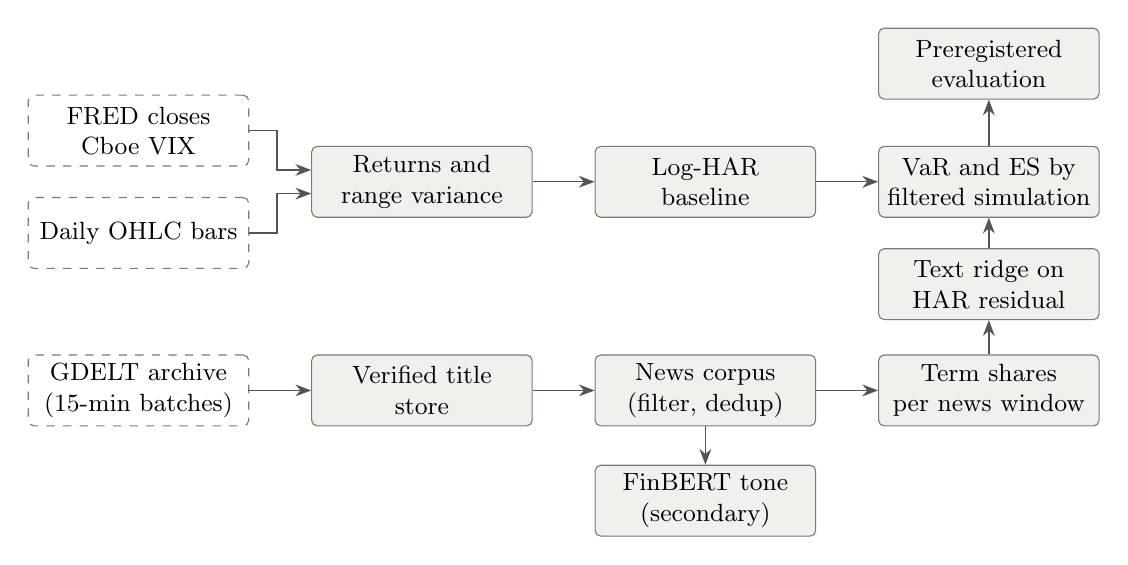
\begin{tikzpicture}[x=1cm, y=1cm,
  box/.style={draw=ink!55, rounded corners=2pt, fill=panel, minimum height=9mm, minimum width=28mm, font=\small, align=center, inner sep=3pt},
  src/.style={box, fill=white, dashed},
  arr/.style={-{Stealth[length=2mm]}, draw=ink!70, line width=0.5pt}]
  \node[src] (fred) at (0,0) {FRED closes\\ Cboe VIX};
  \node[src] (ohlc) at (0,-1.3) {Daily OHLC bars};
  \node[src] (gdelt) at (0,-3.3) {GDELT archive\\ (15-min batches)};
  \node[box] (market) at (3.6,-0.65) {Returns and\\ range variance};
  \node[box] (har) at (7.2,-0.65) {Log-HAR\\ baseline};
  \node[box] (fhs) at (10.8,-0.65) {VaR and ES by\\ filtered simulation};
  \node[box] (eval) at (10.8,0.85) {Preregistered\\ evaluation};
  \node[box] (titles) at (3.6,-3.3) {Verified title\\ store};
  \node[box] (corpus) at (7.2,-3.3) {News corpus\\ (filter, dedup)};
  \node[box] (text) at (10.8,-3.3) {Term shares\\ per news window};
  \node[box] (ridge) at (10.8,-1.95) {Text ridge on\\ HAR residual};
  \node[box] (finbert) at (7.2,-4.7) {FinBERT tone\\ (secondary)};
  \draw[arr] (fred.east) -- ++(0.35,0) |- ([yshift=1.5mm]market.west);
  \draw[arr] (ohlc.east) -- ++(0.35,0) |- ([yshift=-1.5mm]market.west);
  \draw[arr] (market) -- (har);
  \draw[arr] (har) -- (fhs);
  \draw[arr] (fhs) -- (eval);
  \draw[arr] (gdelt) -- (titles);
  \draw[arr] (titles) -- (corpus);
  \draw[arr] (corpus) -- (text);
  \draw[arr] (corpus) -- (finbert);
  \draw[arr] (text) -- (ridge);
  \draw[arr] (ridge) -- (fhs);
\end{tikzpicture}}

\newcommand{\timingdiagram}{%
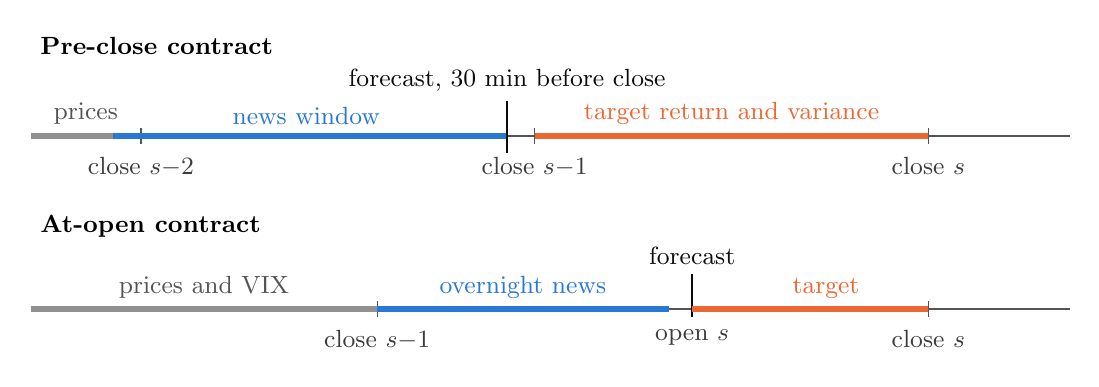
\begin{tikzpicture}[x=1cm, y=1cm, font=\small]
  \def\len{13.2}
  \node[anchor=west, font=\small\bfseries] at (0,2.75) {Pre-close contract};
  \draw[line width=0.6pt, ink!70] (0,1.6) -- (\len,1.6);
  \foreach \x/\lab in {1.4/{close $s{-}2$}, 6.4/{close $s{-}1$}, 11.4/{close $s$}}
    {\draw[ink!70] (\x,1.5) -- (\x,1.7); \node[below, ink!80] at (\x,1.46) {\lab};}
  \draw[ink!45, line width=2.2pt] (0,1.6) -- (1.4,1.6);
  \node[above, ink!70] at (0.7,1.62) {prices};
  \draw[accent, line width=2.2pt] (1.05,1.6) -- (6.05,1.6);
  \node[above, accent] at (3.5,1.62) {news window};
  \draw[ink, line width=0.9pt] (6.05,1.38) -- (6.05,2.05);
  \node[above, ink] at (6.05,2.05) {forecast, 30 min before close};
  \draw[second, line width=2.2pt] (6.4,1.6) -- (11.4,1.6);
  \node[above, second] at (8.9,1.62) {target return and variance};
  \node[anchor=west, font=\small\bfseries] at (0,0.45) {At-open contract};
  \draw[line width=0.6pt, ink!70] (0,-0.6) -- (\len,-0.6);
  \foreach \x/\lab in {4.4/{close $s{-}1$}, 11.4/{close $s$}}
    {\draw[ink!70] (\x,-0.7) -- (\x,-0.5); \node[below, ink!80] at (\x,-0.74) {\lab};}
  \node[below, ink!80] at (8.4,-0.74) {open $s$};
  \draw[ink!45, line width=2.2pt] (0,-0.6) -- (4.4,-0.6);
  \node[above, ink!70] at (2.2,-0.58) {prices and VIX};
  \draw[accent, line width=2.2pt] (4.4,-0.6) -- (8.1,-0.6);
  \node[above, accent] at (6.25,-0.58) {overnight news};
  \draw[ink, line width=0.9pt] (8.4,-0.7) -- (8.4,-0.15);
  \node[above, ink] at (8.4,-0.15) {forecast};
  \draw[second, line width=2.2pt] (8.4,-0.6) -- (11.4,-0.6);
  \node[above, second] at (10.1,-0.58) {target};
\end{tikzpicture}}


\title{\textbf{Does Financial News Improve Daily Risk Forecasts\\ for the S\&P 500?}\\[4pt]
\large Two preregistered studies and a working forecasting system}
\author{Financial News and Daily Market VaR project}
\date{24 November 2026}

\begin{document}
\maketitle

\begin{abstract}
\noindent We test whether financial news improves next-day risk forecasts for the S\&P 500 using
only free data and a CPU. A first study added FinBERT sentiment aggregates to a quantile
regression and found no improvement in 95\% Value-at-Risk. A diagnosis of that failure led to
a second design: forecast volatility first, learn from the data which headline words matter,
and derive Value-at-Risk (VaR) and expected shortfall (ES) from the volatility forecast.
The second study was preregistered and evaluated once on \PooledHoldQlikeN{} sessions from
\HoldoutStart{} to \HoldoutEnd{}. A ridge model of headline terms lowered the volatility
forecast loss of a daily-data baseline (a HAR model with VIX) in both forecast set-ups (pooled
one-sided $p=\HOneP$) and lowered the joint VaR/ES loss (one-sided $p=\HTwoP$). The gains are
modest: \HoldPreQlikeGain{} and \HoldOpenQlikeGain{} in volatility loss and about 1.3--1.5\%
in VaR loss. Generic sentiment scores add little. Two caveats belong next to this result.
About two-thirds of the holdout (December 2023 to December 2025) was the test period of the
first study, whose null result prompted the second design. And on the 224 sessions of 2026,
never evaluated before, the evidence is inconclusive: the pooled volatility gain is not
significant ($t=\PooledFreshQlikeT$) and is negative at the open; the 5\% quantile-loss gain
is nominally significant (one-sided $p=\PooledFreshPinP$, unadjusted) and the joint VaR/ES
gain is not ($p=\PooledFreshFzP$). The result is a working daily forecasting system and a
small, statistically supported but not yet independently confirmed contribution from news text.
\end{abstract}

\section{Question and answer}

\textbf{Question.} Does financial news improve a one-day risk forecast for the S\&P 500 beyond
what market data already provide?

\textbf{Answer.} Yes, modestly, when the news enters as a learned text signal in a volatility
model. No, when it enters as generic sentiment in a quantile regression. The ``yes'' is measured
against a baseline that sees daily prices only, on a holdout whose first two years had served
as the test period of study 1, and it is not yet confirmed on fully untouched data
(Section~\ref{sec:fresh}).

\begin{center}
\begin{tabular}{@{}p{0.30\linewidth}p{0.30\linewidth}p{0.30\linewidth}@{}}
\toprule
 & \textbf{Study 1} & \textbf{Study 2} \\
\midrule
News signal & FinBERT sentiment averages & Ridge model of headline terms \\
Model & 19-feature quantile regression & HAR volatility model, then VaR and ES \\
Test period & 500 sessions, Dec 2023--Dec 2025 & \PooledHoldQlikeN{} sessions, Dec 2023--Nov 2026 \\
Primary result & $-0.06\%$ change in 5\% quantile loss & pooled volatility loss lower, $p=\HOneP$ \\
Registered outcome & not supported & both registered hypotheses passed \\
\bottomrule
\end{tabular}
\end{center}

\section{Data}

All data are free and public. Nothing was purchased and no account was needed.

\begin{center}
\begin{tabular}{@{}p{0.27\linewidth}p{0.66\linewidth}@{}}
\toprule
\textbf{Source} & \textbf{Use} \\
\midrule
FRED, S\&P 500 closes & Close-to-close returns (target of the pre-close set-up) \\
Cboe, VIX closes & Volatility control \\
Yahoo, daily bars for the index and for SPY & Range-based variance; open-to-close return of SPY \\
GDELT Global Knowledge Graph & Page titles of web news, in 15-minute batches \\
\texttt{ProsusAI/finbert} (Dec 2020 revision) & Sentiment scores (study 1; secondary in study 2) \\
\bottomrule
\end{tabular}
\end{center}

\textbf{News.} GDELT was streamed batch by batch from its public archive. Each batch was checked
against the archive's own size and MD5 checksum; only matching titles were kept and the payload
was discarded. Over 2,641 days this transferred about 1.3\,TiB and kept about 1.2\,GiB.
A title is kept when it comes from the web collection, is untranslated, carries the theme
\texttt{ECON\_STOCKMARKET}, mentions a US location and has a usable title. Identical titles or
URLs within 72 hours are dropped in time order. The resulting corpus, from 23 September 2019 to
23 November 2026, has 4.33 million retained events and 4.09 million unique titles.

\textbf{Gaps.} GDELT's archive lacks batches in late 2020, mid 2021 and June 2025. A news window
is used only when at least 95\% of its expected batches were retrieved. A missing batch is never
read as ``no news''.

\textbf{Timing.} GDELT gives the time of a 15-minute batch, not a publication time. A title is
treated as available 15 minutes after its batch. Results are therefore a historical replay with
proxy timestamps, not a record of forecasts issued at the time.

\section{Two forecast set-ups}

\begin{figure}[h]
\centering
\timingdiagram
\caption{Information used and target, for a forecast of session $s$. Grey: market data. Blue:
news. Orange: the period being forecast.}
\end{figure}

The report uses ``set-up'' for a combination of forecast time and target.

\textbf{Pre-close.} The forecast for session $s$ is made 30 minutes before the close of
$s{-}1$. That day's close is not yet known, so market inputs stop at $s{-}2$. The target is the
index return from the close of $s{-}1$ to the close of $s$.

\textbf{At-open.} The forecast is made at the open of session $s$, with market data through the
previous close, the overnight gap, and news that arrived overnight. The target is the
open-to-close return of SPY, the exchange-traded fund that tracks the index. SPY is used
because the index's own value at 09:30 is partly stale: on development data its overnight gap
has only 51\% of the variance of SPY's gap, which would have understated the gap and inflated
the target. An independent reviewer raised this before the test was run.

\section{Method}

\subsection{Volatility target}
Daily variance is measured from price ranges, which is far less noisy than a squared return.
With $O$, $H$, $L$ and $C$ the open, high, low and close of a session, the at-open set-up uses
the Garman--Klass estimator on SPY's bar:
\[
\sigma^2_{\mathrm{GK}} = \tfrac12\left(\ln\tfrac{H}{L}\right)^2-(2\ln 2-1)\left(\ln\tfrac{C}{O}\right)^2 .
\]
For the pre-close set-up we add the squared overnight return of the index. The index's opening
value is partly stale, which shifts some variance between the overnight and intraday parts,
but their sum, which is the target, is roughly preserved.

\subsection{Baseline: HAR with VIX}
The baseline is a log-linear heterogeneous autoregressive (HAR) model \cite{corsi}:
\[
\ln \sigma^2_{s} = \beta_0+\beta_d \ln \sigma^2_{\text{last}}+\beta_w \ln \overline{\sigma^2}_{5}
+\beta_m \ln \overline{\sigma^2}_{22}+\beta_v \ln \mathrm{VIX}^2 \;[+\beta_g\,\text{gap}] + \varepsilon_s ,
\]
with the gap term only at the open. It is refitted by least squares on the first session of each
month, using every earlier session whose outcome was already known.

\subsection{Text model}
Generic sentiment assumes that tone is what matters. Following the idea of news-implied
volatility \cite{nvix}, we let the data choose. Earlier work puts news measures inside volatility models rather than tail regressions \cite{bcp}.
\begin{enumerate}
\item \textbf{Vocabulary.} The 5,000 most frequent one- and two-word terms in titles first seen
by 31 December 2020. It is never updated.
\item \textbf{Features.} For each news window, the share of headlines that contain each term.
This uses every retained headline, with no sampling and no language model.
\item \textbf{Model.} A ridge regression of the baseline's residual on those features. Its
prediction is scaled by a weight estimated from out-of-fold predictions inside the training
data. The weight is zero unless the text beats predicting nothing out of fold.
\end{enumerate}
The final forecast is the baseline plus the scaled text prediction.

\subsection{From volatility to VaR and ES}
Returns are divided by forecast volatility. The 5\% quantile and tail mean of those standardized
returns, taken from past out-of-sample forecasts, are multiplied by the new volatility forecast.
This is filtered historical simulation.

\subsection{Evaluation}
\begin{itemize}
\item \textbf{Volatility:} QLIKE, a standard loss for variance forecasts that is robust to noise
in the variance measure \cite{patton}. Lower is better.
\item \textbf{VaR:} pinball (quantile) loss, in basis points (bp; 1\,bp $=0.01\%$ of return).
\textbf{VaR and ES jointly:} the FZ0 loss \cite{fz,pzc}.
\item \textbf{Tests:} a one-sided Diebold--Mariano test with Newey--West errors \cite{dm} asks
whether the mean daily loss difference favours the text model; its $t$ statistic above 1.65
corresponds to a one-sided $p$ below 0.05. Also: paired moving-block bootstrap intervals; a
conditional predictive ability test \cite{gw}; coverage tests; and the Holm correction when
the two set-ups are tested separately.
\end{itemize}
Only H1 and H2 below were registered as tests. Every other $t$ and $p$ in this report is
unadjusted and exploratory; with five news terms, two set-ups, three losses and three periods,
some would look significant by chance.

\subsection{Preregistration}
Before any study-2 model was evaluated on the holdout (study 1 had already been evaluated on its
first 500 sessions), a record was committed that fixes the inputs by hash,
the source code by content, every model constant, the holdout dates, the hypotheses, the test
and the rule for the verdict (record \texttt{\RegistrationId}). The evaluation command checks
all of these, refuses to run a second time, and wrote its result once.

\begin{quote}
\textbf{H1 (primary).} The text model has lower QLIKE than the baseline, tested once on the
average of the two set-ups' daily improvements.\\
\textbf{H2 (key secondary).} The same for the 5\% FZ0 loss.\\
\textbf{Outcome labels.} \emph{Confirmed} if H1 has one-sided $p<0.05$, both set-ups improve,
and FZ0 does not worsen. \emph{Strong} if H2 also has one-sided $p<0.05$. ``Strong'' names
this rule; it says nothing about the size of the effect.
\end{quote}

\section{Study 1: sentiment in a quantile regression}

The first study scored a 27\% sample of titles with FinBERT, built daily averages of tone and
news volume, and added them to an L1-penalized linear quantile regression with nine market
features. It was preregistered and evaluated once on 500 sessions.

\begin{center}
\begin{tabular}{@{}lrr@{}}
\toprule
\textbf{Model, 5\% tail} & \textbf{Breaches (25 expected)} & \textbf{Mean quantile loss (bp)} \\
\midrule
Market features & 23 & 11.340 \\
+ news counts & 23 & 11.315 \\
+ sentiment & 23 & 11.322 \\
GARCH-$t$ & 26 & 11.890 \\
Historical simulation & 30 & 12.179 \\
\bottomrule
\end{tabular}
\end{center}

Sentiment changed the loss by $-0.06\%$ (95\% interval $-0.022$ to $+0.006$ basis points).
The claim was not supported.

\textbf{Why it failed.} A diagnostic on training and development data only showed that
(i) a 5\% quantile yields 25 breaches in 500 days, too few to detect a small effect;
(ii) negative tone is 0.59 correlated with VIX, which the model already had;
(iii) a one-parameter model, ``quantile $=$ constant $\times$ VIX'', matched the nine-feature
regression, so the model was over-parameterized; and (iv) negative tone did predict next-day
volatility a little after controls ($t=2.9$). That pointed to volatility as the right target.

\section{Study 2: results}

\subsection{Primary test}

\begin{center}
\begin{tabular}{@{}llrrr@{}}
\toprule
\textbf{Period} & \textbf{Loss} & \textbf{Sessions} & \textbf{$t$} & \textbf{One-sided $p$} \\
\midrule
Whole holdout & QLIKE (H1) & \PooledHoldQlikeN & \PooledHoldQlikeT & \PooledHoldQlikeP \\
Whole holdout & 5\% FZ0 (H2) & \PooledHoldFzN & \PooledHoldFzT & \PooledHoldFzP \\
Whole holdout & 5\% pinball & \PooledHoldPinN & \PooledHoldPinT & \PooledHoldPinP \\
\midrule
Dec 2023--2025 & QLIKE & \PooledEarlierQlikeN & \PooledEarlierQlikeT & \PooledEarlierQlikeP \\
2026 (never evaluated) & QLIKE & \PooledFreshQlikeN & \PooledFreshQlikeT & \PooledFreshQlikeP \\
2026 (never evaluated) & 5\% pinball & \PooledFreshPinN & \PooledFreshPinT & \PooledFreshPinP \\
2026 (never evaluated) & 5\% FZ0 & \PooledFreshFzN & \PooledFreshFzT & \PooledFreshFzP \\
\bottomrule
\end{tabular}
\end{center}

Both hypotheses pass on the whole holdout, so the registered outcome is ``\Verdict'' in the
sense defined above. For H1, each set-up also passes by itself after Holm correction
($p=\HolmPre$ pre-close, $p=\HolmOpen$ at-open). H2 passes narrowly; under a two-sided
convention its $p$ would be 0.086. Only the first two rows were registered as tests; the slice
rows are descriptive.

\subsection{By set-up}

\begin{center}
\begin{tabular}{@{}lrrrr@{}}
\toprule
 & \multicolumn{2}{c}{\textbf{Pre-close} (\HoldPreN{} sessions)} & \multicolumn{2}{c}{\textbf{At-open} (\HoldOpenN{} sessions)} \\
\cmidrule(lr){2-3}\cmidrule(lr){4-5}
 & Baseline & Text model & Baseline & Text model \\
\midrule
QLIKE & \HoldPreHarQlike & \HoldPreTextQlike & \HoldOpenHarQlike & \HoldOpenTextQlike \\
5\% pinball loss (bp) & \HoldPreHarPin & \HoldPreTextPin & \HoldOpenHarPin & \HoldOpenTextPin \\
5\% FZ0 loss & \HoldPreHarFz & \HoldPreTextFz & \HoldOpenHarFz & \HoldOpenTextFz \\
5\% breaches (expected) & \HoldPreHarBreaches{} (\HoldPreExpected) & \HoldPreTextBreaches{} (\HoldPreExpected) & \HoldOpenHarBreaches{} (\HoldOpenExpected) & \HoldOpenTextBreaches{} (\HoldOpenExpected) \\
1\% breaches (expected) & \HoldPreHarBreachesOne{} (\HoldPreExpectedOne) & \HoldPreTextBreachesOne{} (\HoldPreExpectedOne) & \HoldOpenHarBreachesOne{} (\HoldOpenExpectedOne) & \HoldOpenTextBreachesOne{} (\HoldOpenExpectedOne) \\
Coverage test $p$ (5\%) & \HoldPreHarKupiec & \HoldPreTextKupiec & \HoldOpenHarKupiec & \HoldOpenTextKupiec \\
\midrule
QLIKE gain of text & \multicolumn{2}{c}{\HoldPreQlikeGain{} ($t=\HoldPreQlikeT$)} & \multicolumn{2}{c}{\HoldOpenQlikeGain{} ($t=\HoldOpenQlikeT$)} \\
5\% pinball gain of text & \multicolumn{2}{c}{\HoldPrePinGain{} ($t=\HoldPrePinT$)} & \multicolumn{2}{c}{\HoldOpenPinGain{} ($t=\HoldOpenPinT$)} \\
\bottomrule
\end{tabular}
\end{center}

Unconditional 5\% coverage is not rejected for the baseline or the text model (Kupiec test).
The dynamic-quantile test, which also looks at clustering of breaches, does not reject either
at 5\%, but rejects both at the 1\% level in the pre-close set-up ($p=0.006$ and $0.013$).
For scale, the baseline's 5\% pinball loss is \HoldPreHarVsHsPin{} (pre-close) and
\HoldOpenHarVsHsPin{} (at-open) lower than that of 250-day historical simulation; on this
holdout those differences are not significant by themselves ($t=1.3$ and $1.5$), though they
were on development data ($t=2.1$ and $2.9$). Historical simulation has 15 breaches at the 1\%
level where about 7 are expected. Most of the system's accuracy comes from the volatility
model; news adds a small further step.

\begin{figure}[h]
\centering
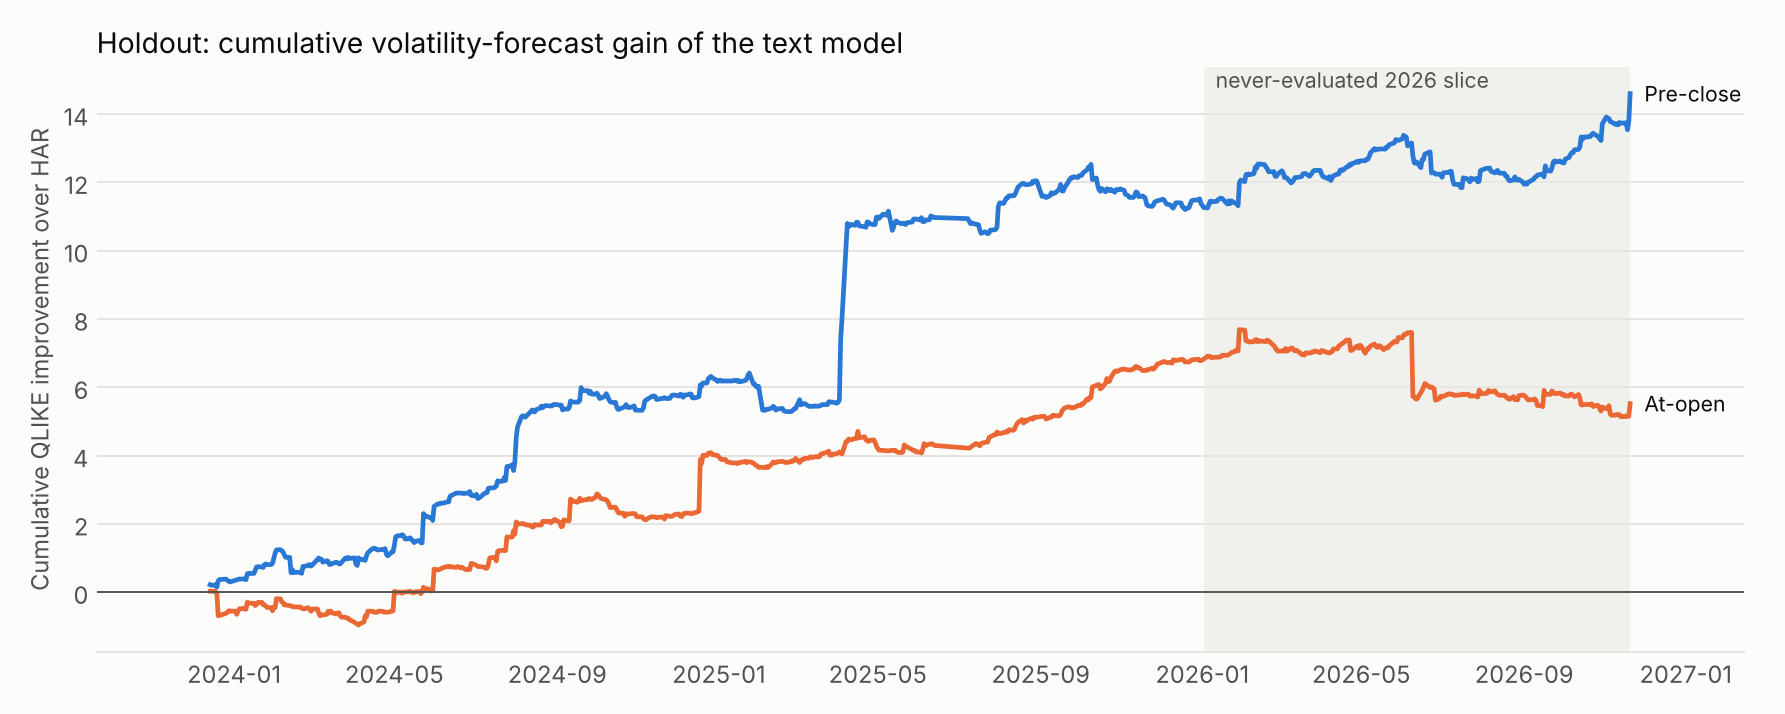
\includegraphics[width=\linewidth]{../docs/figures/vol_cumulative_qlike.png}
\caption{Running total of the text model's daily QLIKE improvement over the baseline.
A rising line means the text model is ahead. Much of the rise comes in a few jumps, the
largest in April 2025, and the at-open line falls in 2026.}
\end{figure}

\subsection{The never-evaluated 2026 slice}\label{sec:fresh}

\begin{center}
\begin{tabular}{@{}lrr@{}}
\toprule
\textbf{2026, 224 sessions} & \textbf{Pre-close} & \textbf{At-open} \\
\midrule
QLIKE gain of text & \FreshPreQlikeGain{} ($t=\FreshPreQlikeT$) & \FreshOpenQlikeGain{} ($t=\FreshOpenQlikeT$) \\
5\% pinball gain of text & \FreshPrePinGain{} ($t=\FreshPrePinT$) & \FreshOpenPinGain{} ($t=\FreshOpenPinT$) \\
\bottomrule
\end{tabular}
\end{center}

This slice is the cleanest evidence, and it is inconclusive.
\begin{itemize}
\item Pooled over both set-ups, the volatility gain is not significant
($t=\PooledFreshQlikeT$). It comes from two days, 29 January and 20 November 2026; without
them the mean is slightly negative ($t=-0.17$).
\item At the open the text model's volatility forecasts are worse than the baseline's in 2026.
\item The 5\% pinball gain is nominally significant when pooled (one-sided
$p=\PooledFreshPinP$, unadjusted), but the registered joint VaR/ES loss is not
($p=\PooledFreshFzP$).
\end{itemize}
With 224 sessions the slice cannot settle the question. It does not contradict the main result
and does not independently confirm it.

\subsection{Which news signal matters}

\begin{figure}[h]
\centering
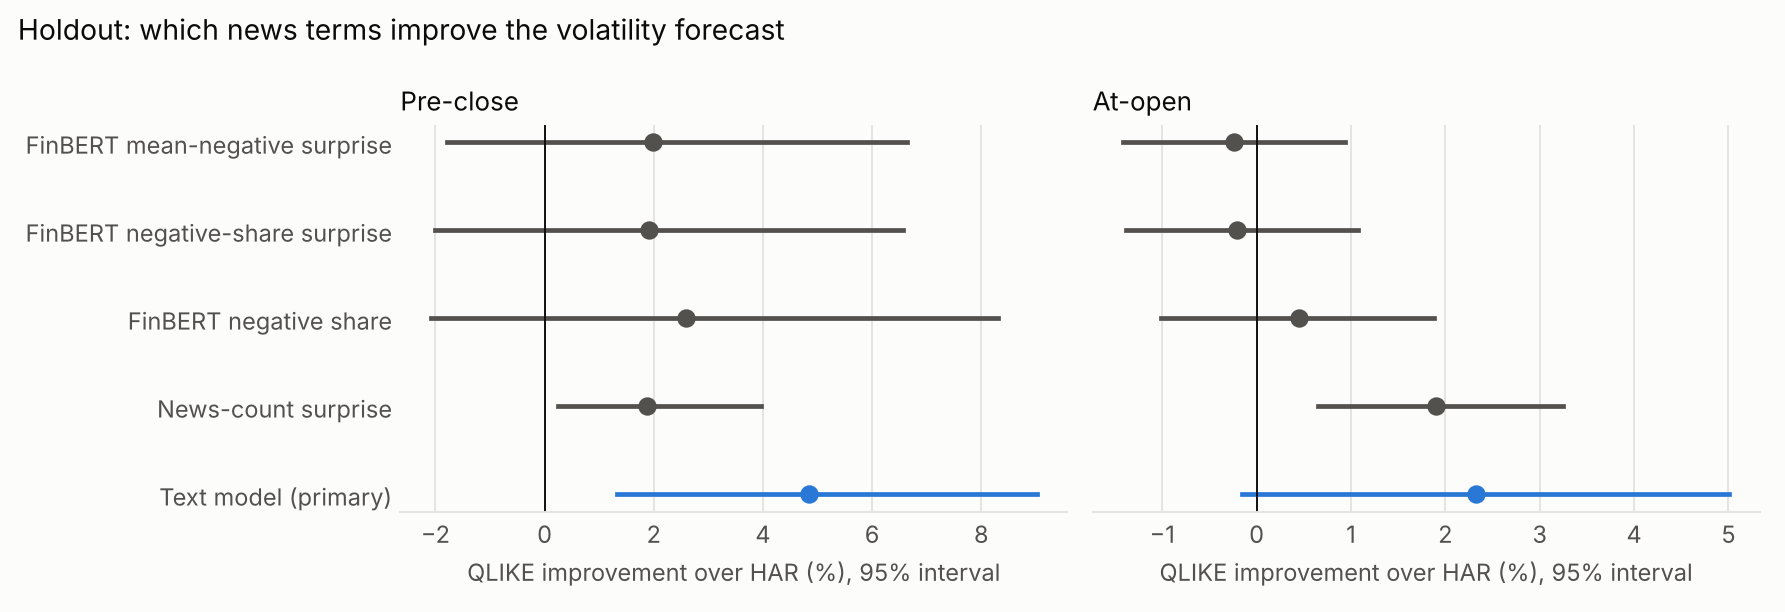
\includegraphics[width=\linewidth]{../docs/figures/vol_gains_by_term.png}
\caption{QLIKE improvement over the baseline on the holdout for each news term, with 95\%
bootstrap intervals. Only the text model was a registered hypothesis. Its gain is the largest
in both set-ups, but its at-open interval includes zero.}
\end{figure}

\begin{itemize}
\item The text model has the largest gains and is the only term that also lowers VaR loss.
Its at-open QLIKE interval includes zero ($t=\HoldOpenQlikeT$).
\item A simple news-volume surprise has smaller QLIKE gains (\HoldPreCountGain{} and
\HoldOpenCountGain) whose intervals exclude zero in both set-ups, but it barely moves VaR
loss. This was exploratory.
\item FinBERT sentiment gives \HoldPreShareSurpriseGain{} pre-close and
\HoldOpenShareSurpriseGain{} at-open, with intervals that include zero. This agrees with study 1.
\end{itemize}

\begin{figure}[h]
\centering
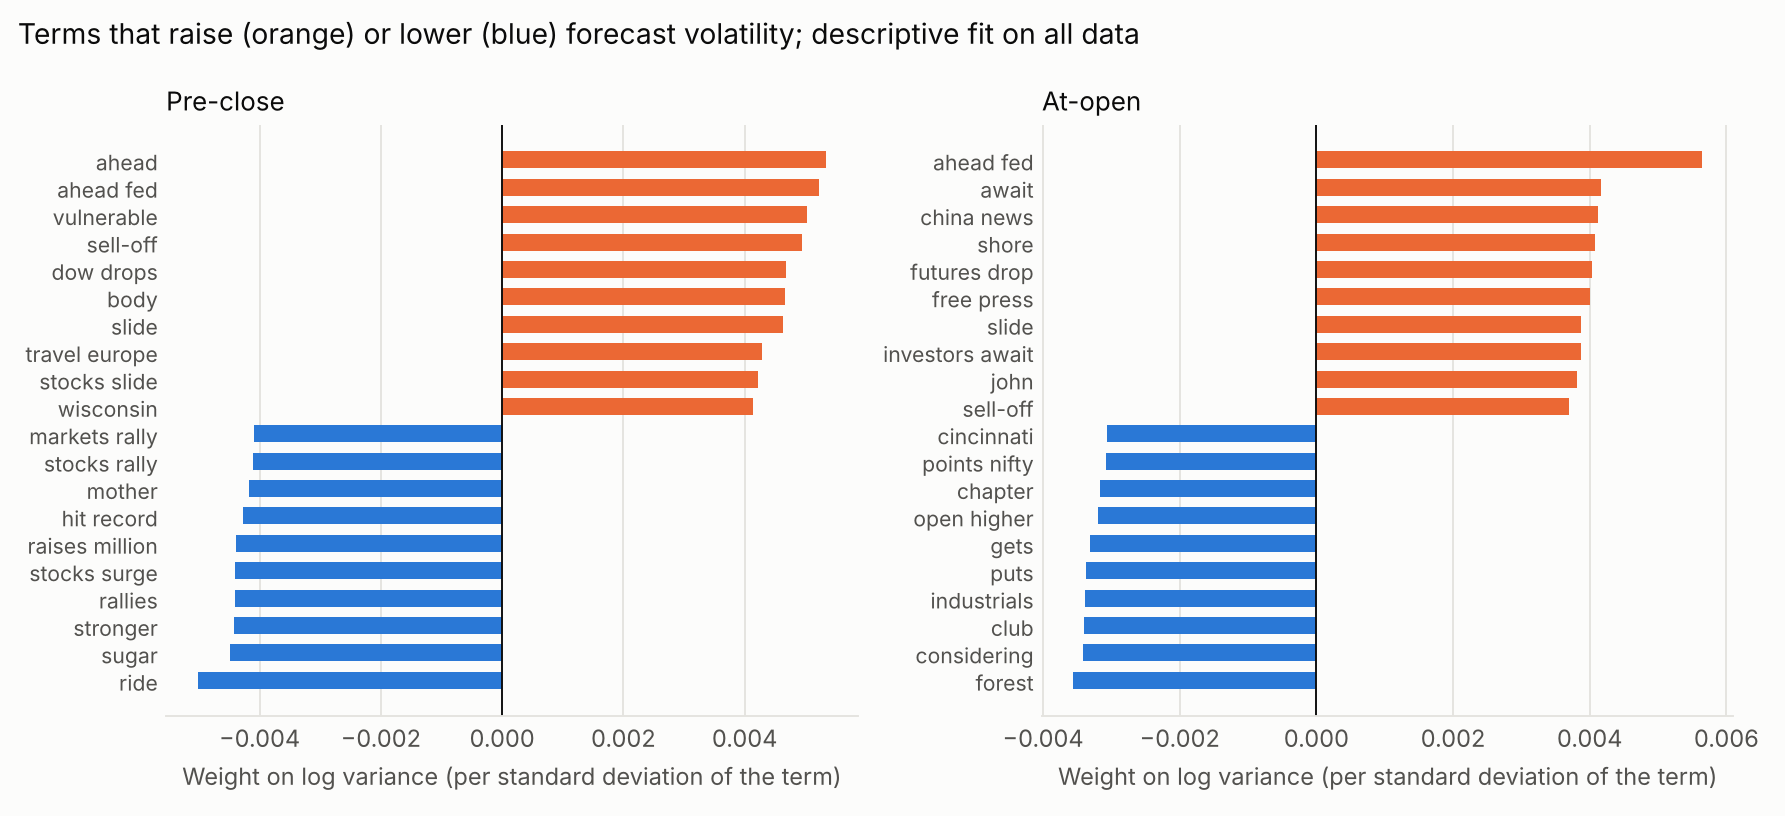
\includegraphics[width=\linewidth]{../docs/figures/vol_term_weights.png}
\caption{Largest term weights from one descriptive fit on all data. Many are sensible
(``ahead fed'', ``sell-off'', ``futures drop'' raise the forecast; ``stocks rally'', ``hit
record'' lower it). Others are noise from an unfiltered web feed (``wisconsin'', ``sugar'').}
\end{figure}

\subsection{Robustness}

These checks were run after the evaluation and are descriptive.
\begin{itemize}
\item \textbf{H1 does not rest on one episode.} April 2025 (the tariff shock) supplies 28\% of
the pooled QLIKE gain. Without that month the pooled QLIKE test still gives $t=2.67$.
\item \textbf{H1 is concentrated in few days.} The seven best days (1\%) supply 53\% of the
net pooled QLIKE gain. Removing the seven best and seven worst days gives $t=4.27$.
The at-open gain is the fragile part: its seven best days supply 88\% of its net gain, and
without them $t=0.26$.
\item \textbf{H2 is fragile.} Without April 2025 the pooled FZ0 test gives $t=1.37$
($p=0.085$); without the single best day, $t=1.60$ ($p=0.055$). Two of the three registered
bootstrap intervals for FZ0 include zero, and neither set-up is significant alone.
\item \textbf{Conditional test.} It rejects equal conditional accuracy in both set-ups
($p=\HoldPreGwP$ and $\HoldOpenGwP$). The statistic includes the unconditional mean, so this
is not separate evidence that the gain varies with market conditions.
\item \textbf{Not a restatement of that day's market.} On development data, giving the pre-close
baseline the same-day variance and VIX, which it cannot have in practice, left the text
model's volatility gain at $+3.4\%$ ($t=3.3$). Its VaR gain shrank from $+2.2\%$ to $+0.6\%$
(\texttt{scripts/oracle\_diagnostic.py}).
\end{itemize}

\begin{figure}[h]
\centering
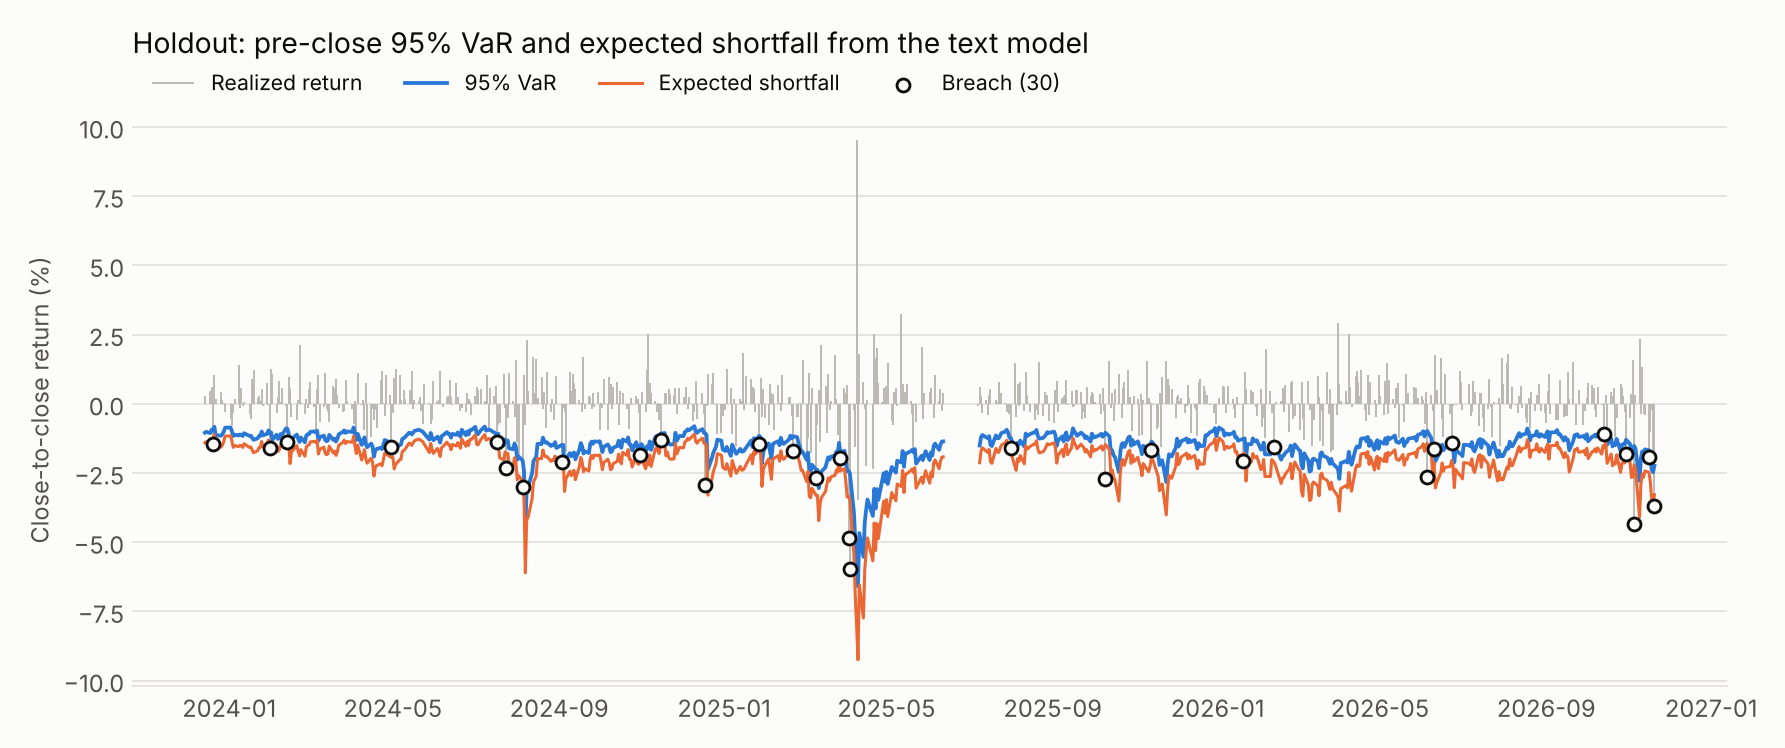
\includegraphics[width=\linewidth]{../docs/figures/vol_var_forecasts.png}
\caption{Pre-close 95\% VaR and expected shortfall from the text model against realized
returns on the holdout. Circles mark breaches. The forecast widens quickly in turbulent periods
and breaches are spread over the period. The line breaks where GDELT has no data.}
\end{figure}

\section{Limits}

\begin{enumerate}
\item \textbf{The effect is small and partly fragile.} Volatility loss falls 2--5\% and VaR
loss about 1.5\%. The volatility result (H1) survives the robustness checks; the VaR/ES result
(H2) and the at-open volatility gain do not survive all of them.
\item \textbf{Part of the holdout was used before.} December 2023 to December 2025 was the test
period of study 1, and that study's failure prompted this design. No volatility or text model
had been evaluated there, but the design is not blind to that period. The 2026 slice is fully
clean and is inconclusive.
\item \textbf{The baseline uses daily data only.} In the pre-close set-up headlines run to
15:30 while prices stop at the previous close. The result shows that news text improves a
daily-data model. It does not show that news beats intraday prices, which were not available.
\item \textbf{Noisy source.} GDELT titles are web page titles, not curated financial headlines.
In an audit of 200 titles from 2019--2022, chosen in equal numbers by FinBERT label rather than
at random, about one in seven was off-topic. The audit was rated by the project's AI agent,
not by a human, and the individual ratings were not archived.
\item \textbf{Proxy timestamps.} See Section 2.
\item \textbf{Design choices were made on development data.} Five news terms, two penalty grids,
two feature forms and two price sources were compared there, and are all listed in the research
log. One of them, the penalty grid, changes the development result noticeably.
\item \textbf{The 1\% tail} is not significantly improved by news and has too few breaches to
say much.
\item \textbf{Many comparisons.} Apart from H1 and H2, every $t$ and $p$ here is unadjusted.
\item \textbf{No human review.} The work, the audit and the reviews were done by AI agents.
\end{enumerate}

\section{The system}

\begin{figure}[h]
\centering
\pipelinediagram
\caption{Pipeline. Dashed boxes are external sources.}
\end{figure}

The project is a Python package, \texttt{newsvar}, with a command-line interface. Every stage
writes a checksummed, content-addressed artifact and can be resumed.

\begin{center}
\begin{tabular}{@{}p{0.30\linewidth}p{0.63\linewidth}@{}}
\toprule
\textbf{Command} & \textbf{What it does} \\
\midrule
\texttt{newsvar update} & Refreshes prices, the calendar, GDELT titles, the corpus and scores (about 5 minutes) \\
\texttt{newsvar forecast} & Issues volatility, VaR and ES for the next session and appends to a log \\
\texttt{newsvar vol develop / preregister / evaluate / report} & The staged, gated study \\
\texttt{newsvar gdelt extract}, \texttt{news corpus}, \texttt{news score} & The data stages \\
\bottomrule
\end{tabular}
\end{center}

\textbf{A demonstration run.} On 24 November 2026 at 14:51 New York time, after both forecast
times for that session had passed, the system produced for that day's session a 95\% VaR of
$-3.5\%$ and ES of $-5.2\%$ (pre-close set-up, index close-to-close) and a 95\% VaR of
$-2.4\%$ (at-open set-up, SPY open-to-close). The pre-close forecast used the VIX close of
20 November (35.9); the at-open forecast that of 23 November (26.6). This entry shows that the
commands work; it is not a prospective forecast.

\textbf{Resources.} Everything ran on four CPU cores and 15\,GiB of memory: about three hours to
stream the news archive, five hours to score titles with FinBERT (not needed by the text
model), and minutes for everything else.

\textbf{Quality control.} The code has 105 automated tests on synthetic data, including tests
that changing future data cannot change an earlier forecast. Two AI reviewer agents, started by
the project's own AI agent and working read-only, audited the second study before its test was
run. They found no look-ahead; they did find a stale opening price, a mis-sized test, in-sample
tail estimates and weak registration checks, all of which were fixed before registration.
Two more reviewed the finished project: one audited every number and claim in this report
against the records and made it more cautious in several places (the fragility of H2, the
2026 slice, coverage wording); the other audited the code and the operational commands.
No human has reviewed the work.

\section{Conclusion}

A free, noisy news feed does carry a little information about tomorrow's risk that a good
daily-data volatility model lacks. It shows up when the model is allowed to learn which words
matter and when the target is volatility; it does not show up as generic sentiment in a tail
regression. The evidence meets a preregistered standard on the whole holdout and is
inconclusive on the one fully clean year.

The practical value today is the forecasting system itself: a VaR and ES forecaster with
acceptable 5\% coverage and lower loss than historical simulation (4.7\% and 9.9\% on the
holdout, not significant there by themselves), with a small news component on top.

\textbf{What would strengthen the claim.} (i) Keep logging forecasts prospectively: every new
session is clean evidence with real timestamps. (ii) Test a curated headline feed with a longer
history. (iii) Add intraday prices to the baseline to see whether news survives.

\begin{thebibliography}{9}\small
\bibitem{corsi} F.~Corsi (2009). A simple approximate long-memory model of realized volatility. \emph{Journal of Financial Econometrics}.
\bibitem{nvix} A.~Manela and A.~Moreira (2017). News implied volatility and disaster concerns. \emph{Journal of Financial Economics} 123, 137--162.
\bibitem{patton} A.~Patton (2011). Volatility forecast comparison using imperfect volatility proxies. \emph{Journal of Econometrics}.
\bibitem{fz} T.~Fissler and J.~Ziegel (2016). Higher order elicitability and Osband's principle. \emph{Annals of Statistics}.
\bibitem{pzc} A.~Patton, J.~Ziegel and R.~Chen (2019). Dynamic semiparametric models for expected shortfall (and Value-at-Risk). \emph{Journal of Econometrics}.
\bibitem{dm} F.~Diebold and R.~Mariano (1995). Comparing predictive accuracy. \emph{Journal of Business \& Economic Statistics}.
\bibitem{gw} R.~Giacomini and H.~White (2006). Tests of conditional predictive ability. \emph{Econometrica} 74, 1545--1578.
\bibitem{bcp} M.~Bernardi, L.~Catania and L.~Petrella (2017). Are news important to predict large losses? \emph{European Journal of Finance}.
\end{thebibliography}
\end{document}
